\begin{figure}[t]
    \centering
        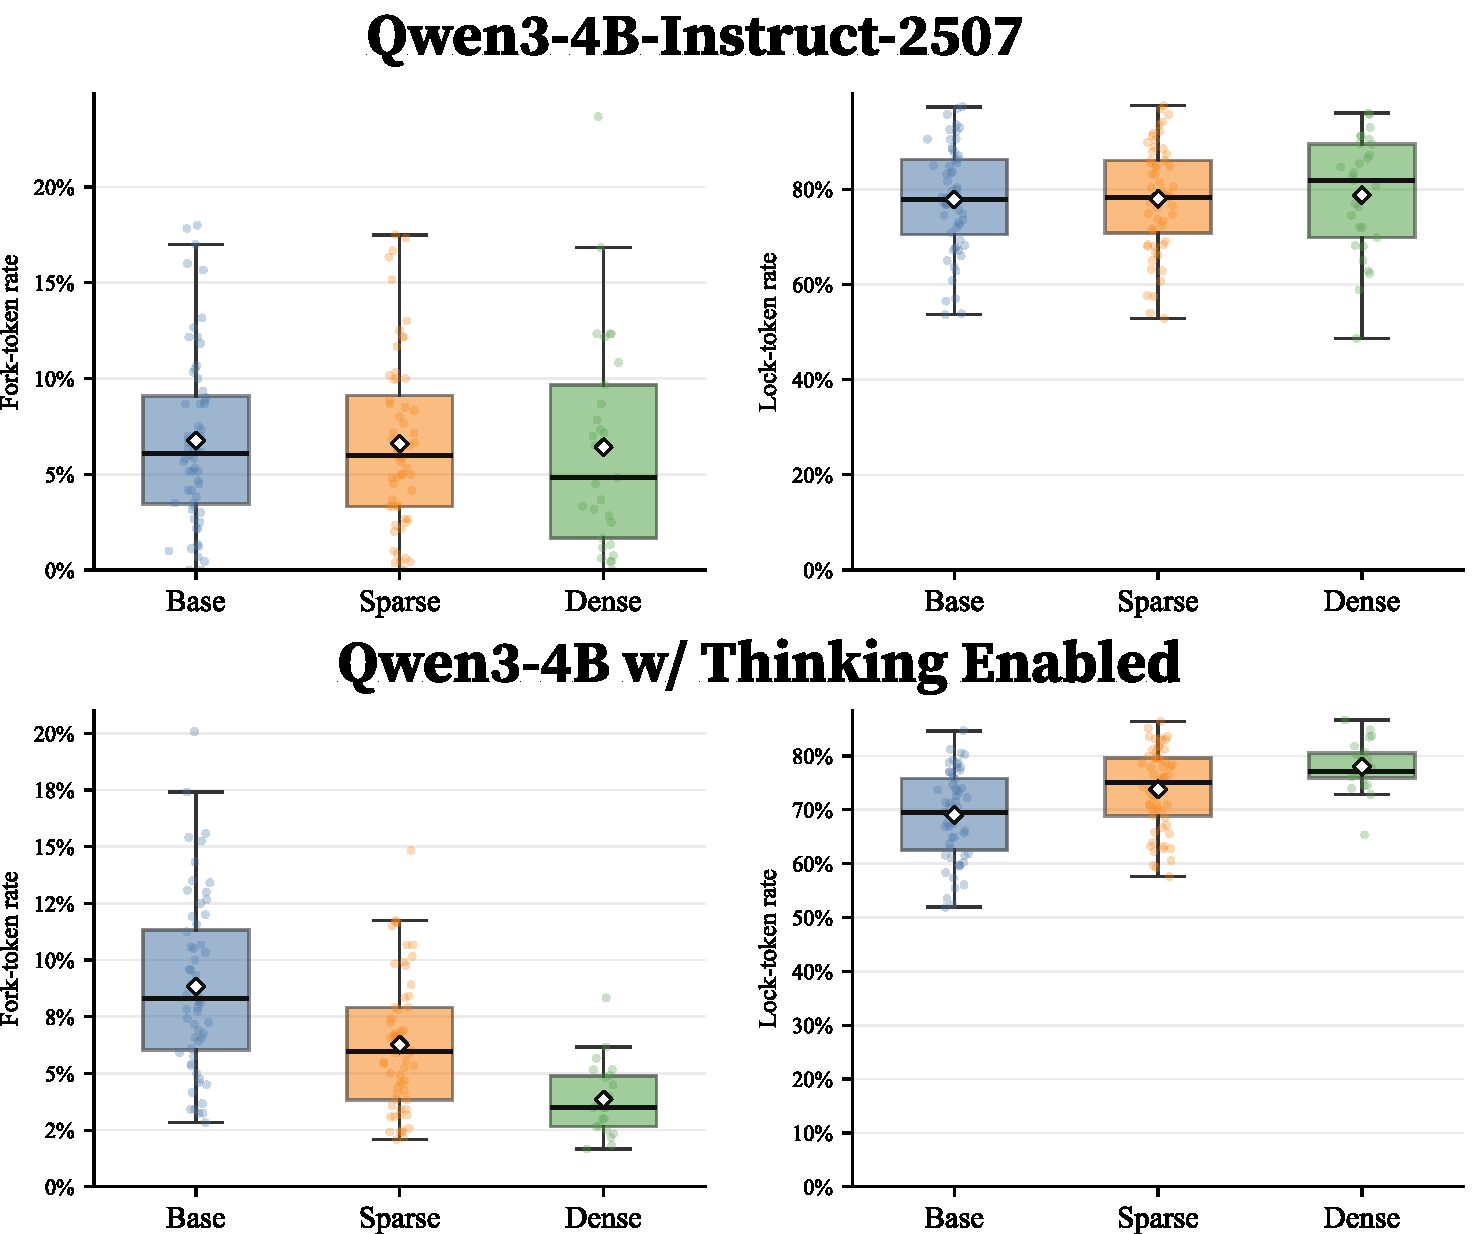
\includegraphics[width=\linewidth]{figures/qwen3-4b-qwen3-4b-instruct-2507__fork_lock_rate_boxplots.pdf}
    \caption{
    \textbf{Dense privileged context lowers fork rates in thinking rollouts but has little effect on instruction-style rollouts.}
    We compute fork and lock rates using the SSD-style diagnostic of \citet{zhang2026embarrassingly}: fork positions are high-entropy decision points with multiple plausible continuations, while lock positions are locally determined continuations. Panels show the \opsd{} side of the diagnostic for base, sparse privileged-context, and dense privileged-context conditions; the left column shows fork rate and the right column shows lock rate. For the instruction-tuned model, fork and lock rates remain mostly flat as privileged context becomes denser, with at most a small dense-context reduction in fork rate. For the thinking model, denser privileged context lowers fork rate and raises lock rate, consistent with the hypothesis that \opsd{} suppresses the branching points needed for test-time search.
    }
    \label{fig:fork_lock_context}
\end{figure}
